% Figure from MATH 556 notes, section 7. Compile with the notes preamble.
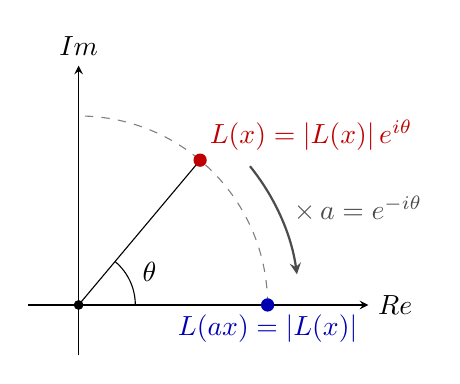
\begin{tikzpicture}[scale=1.6, >=stealth]
    \draw[->] (-0.4,0) -- (2.3,0) node[right] {$\operatorname{Re}$};
    \draw[->] (0,-0.4) -- (0,1.9) node[above] {$\operatorname{Im}$};
    \draw[dashed, gray] (1.5,0) arc (0:90:1.5);
    \coordinate (L) at (50:1.5);
    \draw[thin] (0,0) -- (L);
    \fill[red!75!black] (L) circle (1.5pt) node[above right, red!75!black] {$L(x) = |L(x)|\,e^{i\theta}$};
    \draw (0.45,0) arc (0:50:0.45);
    \node at (25:0.62) {$\theta$};
    \fill[blue!70!black] (1.5,0) circle (1.5pt) node[below, blue!70!black] {$L(ax) = |L(x)|$};
    \draw[->, thick, gray!60!black] (39:1.75) arc (39:8:1.75);
    \node[gray!60!black, anchor=west] at (25:1.8) {$\times\, a = e^{-i\theta}$};
    \fill (0,0) circle (1.1pt);
\end{tikzpicture}
